\documentclass{beamer}

\usepackage[utf8]{inputenc}
\usepackage{listings}
\usetheme{Copenhagen}
\setbeamertemplate{navigation symbols}{}
\setbeamertemplate{headline}{}
\setbeamertemplate{footline}{}

\title{Map Abstraction for Multi-Agent Pathfinding problems with Answer Set Programming}
\author[Adrian Salewsky]{Adrian Salewsky}
\institute{University of Potsdam}
\date{23.06.2022}

\begin{document}

\frame{\titlepage}

\begin{frame}
\frametitle{Table of Contents}
\tableofcontents
\end{frame}

\section{Introduction} 
\begin{frame}
\frametitle{Introduction}
\begin{itemize}
\item<2-> Reducing map size to increase speed
\medskip
\item<3-> Predetermined goal coordinates
\medskip
\item<4-> Three methods to achieve goal
\medskip
\item<5-> Asprilo as base
\end{itemize}
\end{frame}

\begin{frame}
\frametitle{Introduction}
\begin{figure}[h]
\centering{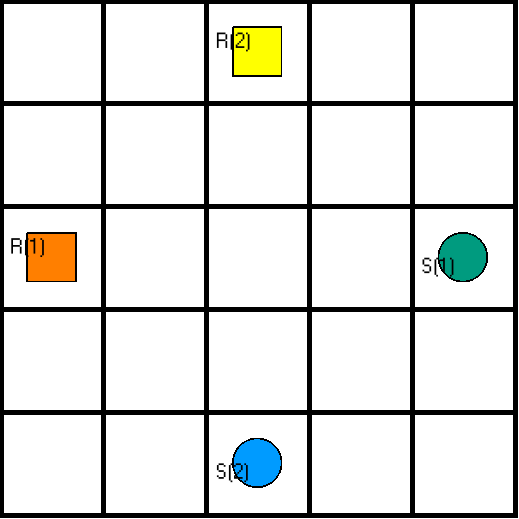
\includegraphics[scale=.4]{Images/MAPF-Problem}}
\end{figure}
\end{frame}

\section{Abstraction Methods}
\begin{frame}
\frametitle{Shortest Path}
\begin{itemize}
\item<2-> Looking for shortest path of each robot
\medskip
\item<3-> Conflicts between robots are ignored
\medskip
\item<4-> Every node not visited gets deleted
\medskip
\item<5-> Remaining nodes are output
\end{itemize}
\end{frame}

\begin{frame}
\frametitle{Shortest Path}
\begin{figure}[h]
\centering{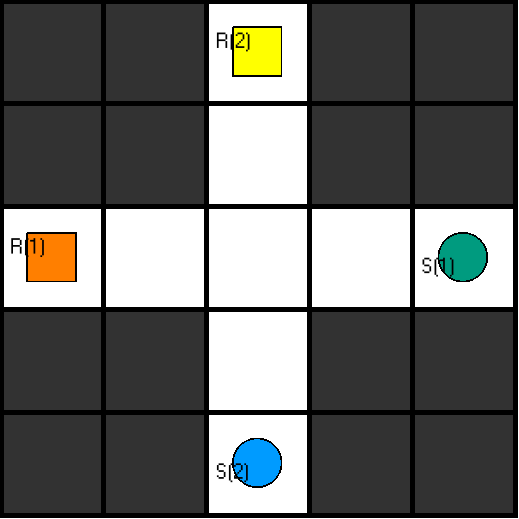
\includegraphics[scale=.4]{Images/SP-Example}}
\end{figure}
\end{frame}

\begin{frame}
\frametitle{Node Combining}
\begin{itemize}
\item<2-> Multiple nodes are combined
\medskip
\item<3-> Finding shortest path in smaller map
\medskip
\item<4-> Nodes that were visited in their combined form are kept
\medskip
\item<5-> Open Node Combining for open maps
\item<6-> Complete Node Combining for maps with walls
\end{itemize}
\end{frame}

\begin{frame}
\frametitle{Node Combining}
\begin{figure}[h]
\centering{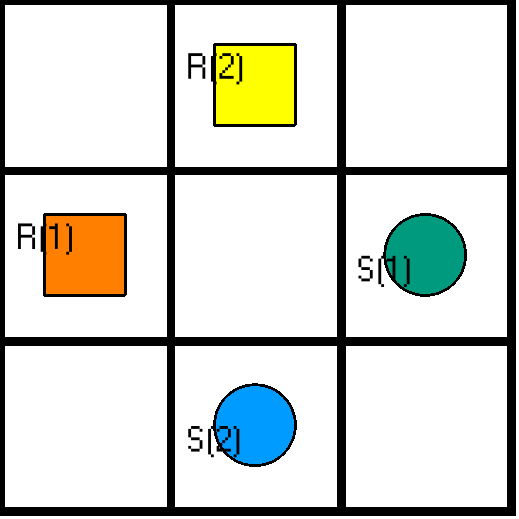
\includegraphics[scale=.4]{Images/Post-Combining-Example}}
\end{figure}
\end{frame}

\begin{frame}
\frametitle{Node Combining}
\begin{figure}[h]
\centering{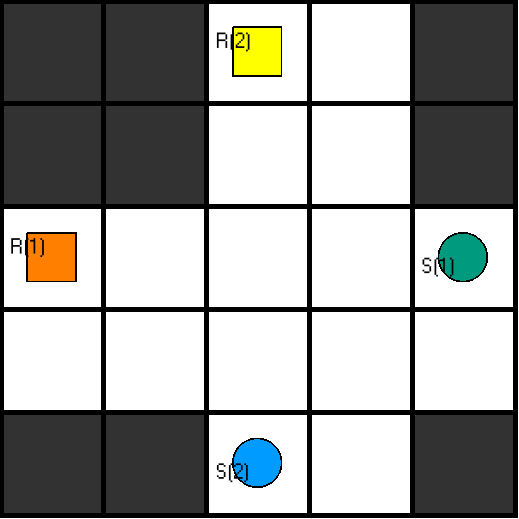
\includegraphics[scale=.4]{Images/ONC-2-2-Example}}
\end{figure}
\end{frame}

\begin{frame}
\frametitle{Reachable Nodes}
\begin{itemize}
\item<2-> Shortest path for each robot
\medskip
\item<3-> Calculating the amount of steps each node is deviating from the shortest path
\medskip
\item<4-> Maximum number of deviating steps is the individual makespan
\medskip
\item<5-> Output contains the information about the number of deviating steps
\end{itemize}
\end{frame}

\begin{frame}
\frametitle{Reachable Nodes}
\begin{figure}[h]
\centering{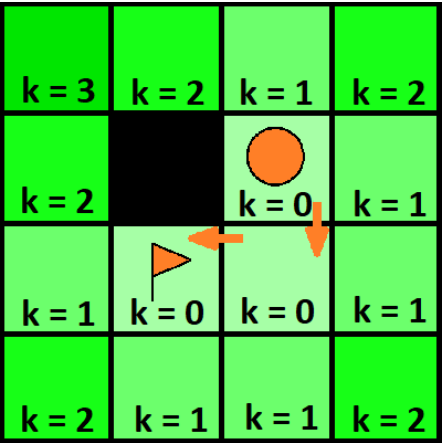
\includegraphics[scale=.4]{Images/RN-Explanation}}
\end{figure}
\end{frame}

\section{Auxiliary Programs}
\begin{frame}
\frametitle{Auxiliary Programs}
\begin{itemize}
\item<2-> Multiple python programs for easier use
\medskip
\item<3-> Map generator for creating open maps
\medskip
\item<4-> Multiple solvers using incrementation for horizon
\medskip
\item<5-> Result plotters for analyzing benchmark results
\end{itemize}
\end{frame}

\section{Benchmarking}
\begin{frame}
\frametitle{Benchmarking}
\begin{itemize}
\item<2-> Shortest Path and Reachable Nodes are worse than asprilo
\medskip
\item<3-> Especially Reachable Nodes has performance issues
\medskip
\item<4-> Node Combining can beat asprilo in certain scenarios
\medskip
\item<5-> Using the right size for Node Combining is important
\end{itemize}
\end{frame}

\section{Conclusion}
\begin{frame}
\frametitle{Conclusion}
\begin{itemize}
\item<2-> Goal: Achieving time improvement for MAPF-Problems
\medskip
\item<3-> Method: Decreasing node count to have faster solving
\medskip
\item<4-> Three different abstraction methods
\medskip
\item<5-> Node Combining shows promise
\end{itemize}
\end{frame}

\end{document}